\documentclass[12pt]{article}
\usepackage{graphics}
\begin{document}
\newcounter{problem}
\thispagestyle{empty}

% must be shortened...

\section*{NYU Physics 1---Problem set 11}

Due Tuesday 2009 December 8 at the beginning of lecture.

\paragraph{Problem~\theproblem:}\refstepcounter{problem}%
A toy car has a \emph{total} mass of 50~g, and rolls on freely
spinning wheels, each of which can be modeled as a uniform disk of
mass 1~g and radius 2~mm.  What is the acceleration $a$ of this toy
car when it rolls without slipping down a ramp tilted at an angle of
20~deg to the horizontal?  By what factor is the toy car faster or
slower than a frictionless block of the same total mass, \textit{ie,}
what is $a_\mathrm{car}/a_\mathrm{frictionless}$?

\paragraph{Problem~\theproblem:}\refstepcounter{problem}%
A thin, uniform beam of mass $m_\mathrm{b}$ and length $L_x$ is
attached to a wall by a pivot and a wire, as shown.  The beam supports
a sign of mass $m_\mathrm{s}$.
\\ \rule{0.35\textwidth}{0pt}
\resizebox{0.3\textwidth}{!}{\includegraphics{../mp/hanging_sign.eps}}
\\
Find the tensions $T_1$ and $T_2$ in the two wires and the vector
force $\vec{F}$ on the beam at the pivot, in terms of the quantities
shown and the acceleration $g$ due to gravity.  Assume that the pivot
is frictionless (so it provides no torque) and that the wires are
massless.  If there was friction on the pivot, what parts of your
answer would change, and in which direction?

\paragraph{Problem~\theproblem:}\refstepcounter{problem}%
\textsl{(a)}~A hockey puck (a uniform disk of mass $m$, radius $r$,
and thickness $t$), slides without friction on ice with initial speed
$v_0$.  It strikes an identical puck tangentially, as shown in the
figure, and sticks to it.  The second puck is initially at rest and
also can slide without friction.  What is the final (linear) velocity
(speed $v$ and direction) of the stuck-together pucks?  What is the
moment of inertia $I_f$ and final angular speed of rotation $\omega$
of the system around its center of mass?  What fraction of the initial
kinetic energy (if any) is lost; \textit{ie,} what is $[K_i-K_f]/K_i$?
\\ \rule{0.25\textwidth}{0pt}
\resizebox{0.50\textwidth}{!}{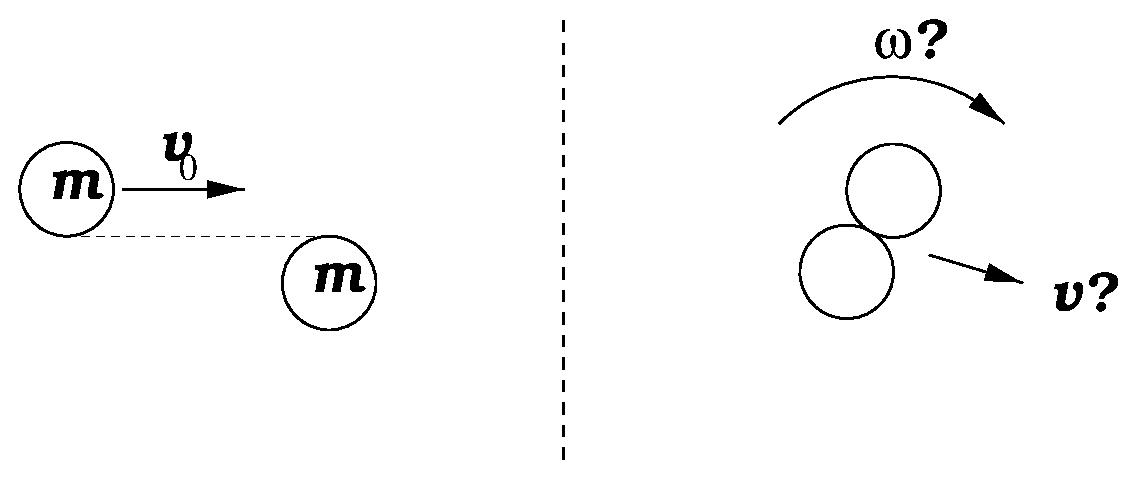
\includegraphics{../eps/tangpucks.eps}}
\\
\emph{Draw a clear diagram with a clearly labeled reference point used
to compute the angular momentum; recall that any angular momentum
calculation is with respect to your chosen origin.}

\textsl{(b)}~If the pucks had hit dead-on, the stuck-together pucks,
after the collision, would not be rotating.  Which of your answers
($v$, $\omega$, and $[K_i-K_f]/K_i$) will be different in this case?
If the fractional loss in kinetic energy is different, explain where
the difference in energy went.

\paragraph{Extra Problem (will not be graded for credit):}%
Hogg problem~6--8.  The ``$p$'' in the problem statement is the
magnitude of the momentum of either particle 1 or 2.  Solve for $p$
and $E_1$ as a function of $M$ and $m_1$ and only after you have done
so, take the limit $m_1\rightarrow 0$.

\end{document}
